\newpage

\title{Блок-схема}{\begin{center}
    Блок-схема
\end{center}} \\
\begin{figure}[H]
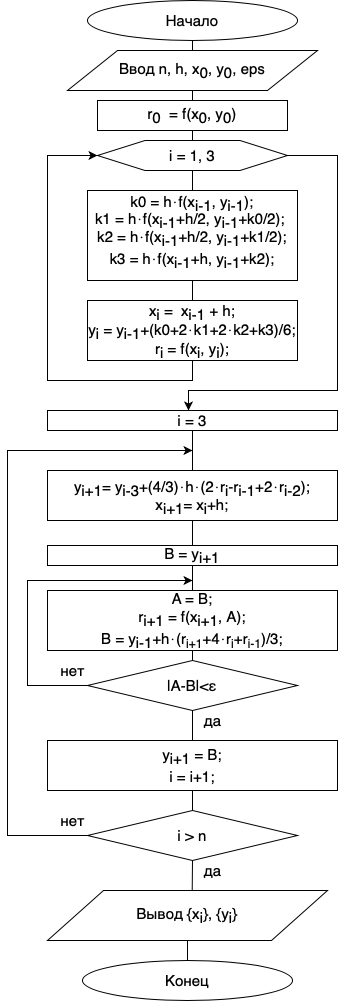
\includegraphics[width = 0.48\textwidth]{comp-math-lab4.png}
 
\end{figure} 

\newpage

\title{Листинг численного метода}{\begin{center}
    Листинг численного метода
\end{center}} \\
    \begin{verbatim}
        
//  RungeKuttaMethod.java
    public RungeKuttaMethod(double x0, double y0, double xn, 
            double accuracy, Function function) {
//        this.step = Math.pow(accuracy, 0.25);
        this.step = accuracy;
        this.function = function;
        values = new ArrayList<>();
        values.add(new Pair<>(x0, y0));
        double y_next = y0;
        for (double i = x0; i < xn; i += step) {
            y_next = getNextYValue(i, y_next);
            values.add(new Pair<>(i+step, y_next));
        }
    }

    private double getNextYValue(double x, double y) {
        double k0, k1, k2, k3, delta;
        k0 = function.getValue(x, y);
        k1 = function.getValue(x + step/2, y + k0 * step/2);
        k2 = function.getValue(x + step/2, y + k1 * step/2);
        k3 = function.getValue(x + step, y + k2 * step);
        delta = step * (k0 + 2 * k1 + 2 * k2 + k3)/6;
        return y + delta;
    }
    
//  MilneMethod.java
   public MilneMethod(double x0, double y0, double xn, double accuracy, 
            Function function) {
        values = new RungeKuttaMethod(x0, y0, xn, accuracy, function).
            getValues(4);
        this.function = function;
//        this.step = Math.pow(accuracy, 0.25);
        this.step = accuracy;
        this.accuracy = accuracy;
        this.xn = xn;
        this.currentX = x0 + 3 * this.step;
        calculate();
    }

    private void calculate() {
        int i = 3;
        while (currentX < xn) {
            i ++;
            currentX += step;
            double f3, f2, f1, f;
            f3 = function.getValue(values.get(i - 3).getKey(),
                    values.get(i - 3).getValue());
            f2 = function.getValue(values.get(i - 2).getKey(),
                    values.get(i - 2).getValue());
            f1 = function.getValue(values.get(i - 1).getKey(),
                    values.get(i - 1).getValue());
            f = function.getValue(values.get(i - 1).getKey() + step,
                    values.get(i - 4).getValue() +
                            4 * step * (2 * f3 - f2 + 2 * f1)/3);
            double y = f;
            do {
                f = y;
                y = values.get(i - 2).getValue() + step*(f + 4 * f1 + f2)/3;
            } while (Math.abs(f - y)/29 > accuracy);
            values.add(new Pair<>(values.get(i - 1).getKey()+step, y));
        }
    }
     \end{verbatim}
\newpage

\title{Примеры}{\begin{center}
    Примеры
\end{center}} \\
\begin{figure}[H]
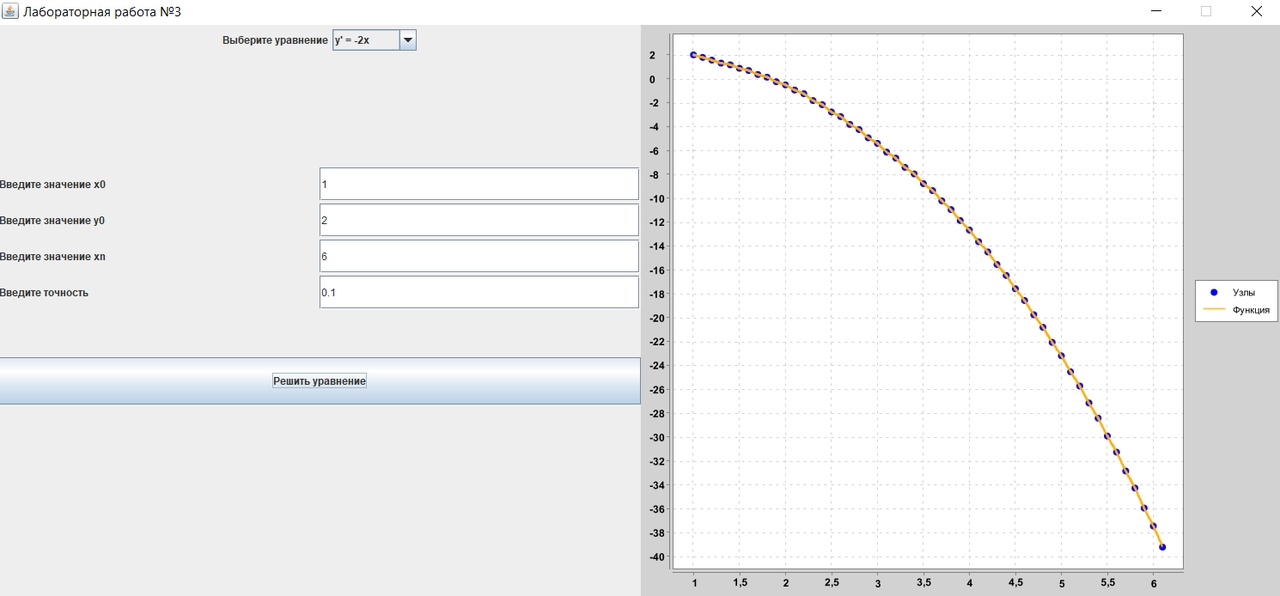
\includegraphics[width = 1\textwidth]{0.png}
\end{figure} 

\begin{figure}[H]
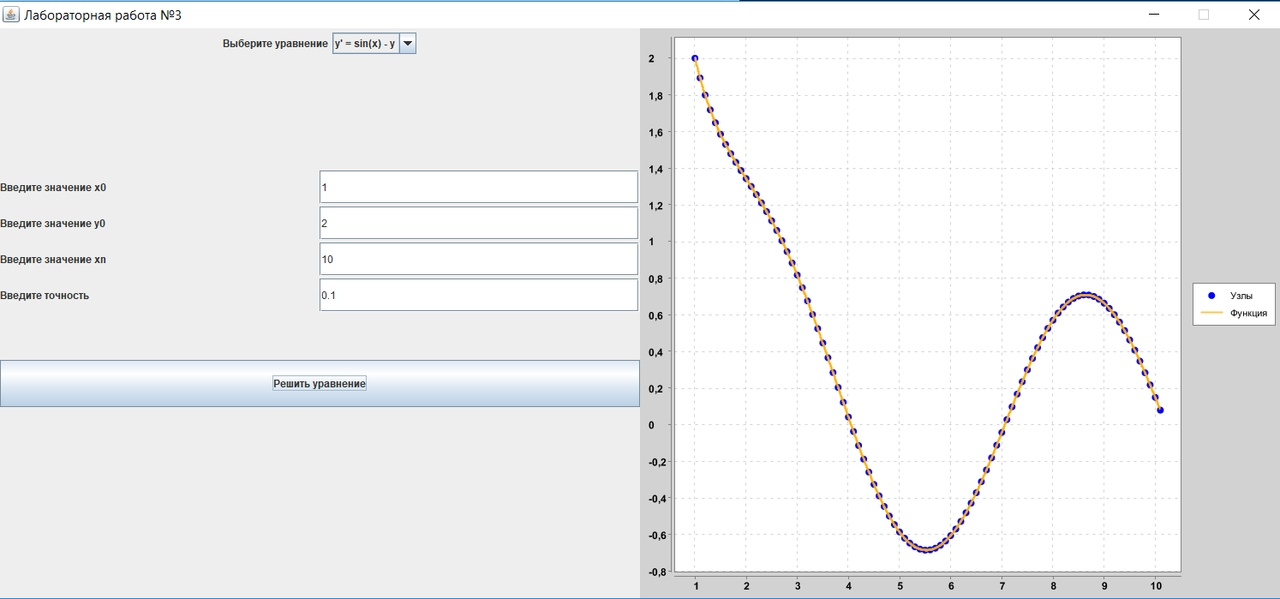
\includegraphics[width = 1\textwidth]{1.png}
\end{figure} 

\begin{figure}[H]
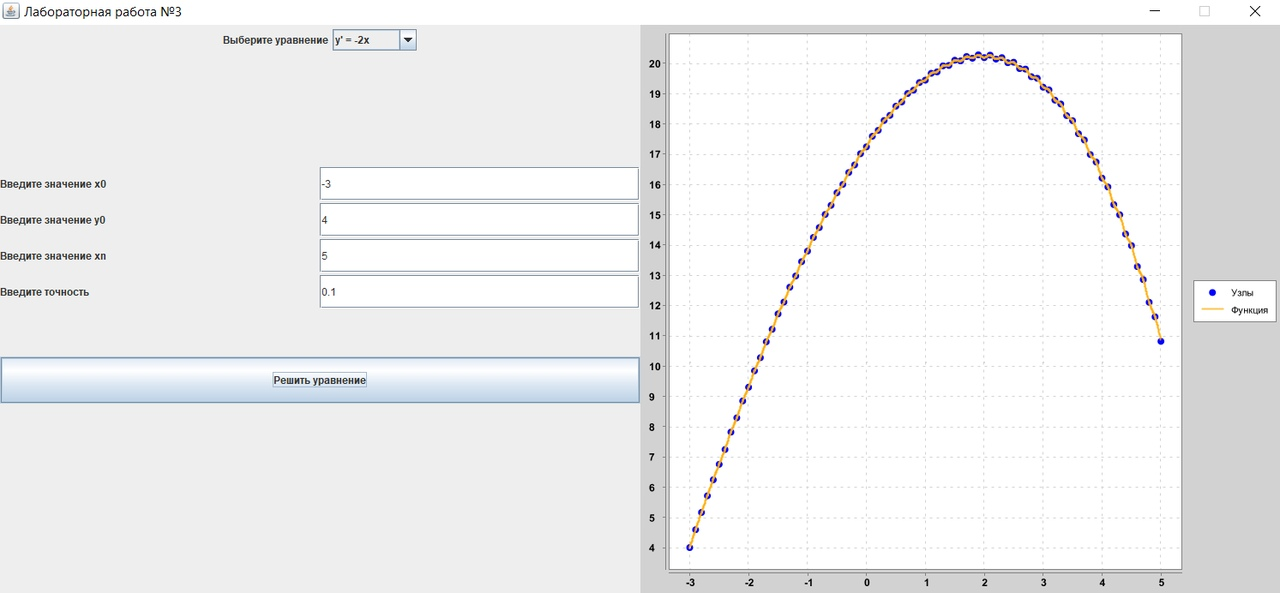
\includegraphics[width = 1\textwidth]{2.png}
\end{figure} 
